\documentclass{mimosis}

\usepackage{metalogo}
\setlength{\parindent}{0pt}

%%%%%%%%%%%%%%%%%%%%%%%%%%%%%%%%%%%%%%%%%%%%%%%%%%%%%%%%%%%%%%%%%%%%%%%%
% Some of my favourite personal adjustments
%%%%%%%%%%%%%%%%%%%%%%%%%%%%%%%%%%%%%%%%%%%%%%%%%%%%%%%%%%%%%%%%%%%%%%%%
%
% These are the adjustments that I consider necessary for typesetting
% a nice thesis. However, they are *not* included in the template, as
% I do not want to force you to use them.

% This ensures that I am able to typeset bold font in table while still aligning the numbers
% correctly.
\usepackage{etoolbox}

\usepackage[binary-units=true]{siunitx}
\DeclareSIUnit\px{px}

\sisetup{%
  detect-all           = true,
  detect-family        = true,
  detect-mode          = true,
  detect-shape         = true,
  detect-weight        = true,
  detect-inline-weight = math,
}

%%%%%%%%%%%%%%%%%%%%%%%%%%%%%%%%%%%%%%%%%%%%%%%%%%%%%%%%%%%%%%%%%%%%%%%%
% Hyperlinks & bookmarks
%%%%%%%%%%%%%%%%%%%%%%%%%%%%%%%%%%%%%%%%%%%%%%%%%%%%%%%%%%%%%%%%%%%%%%%%

\usepackage[%
  colorlinks = true,
  citecolor  = RoyalBlue,
  linkcolor  = RoyalBlue,
  urlcolor   = RoyalBlue,
  ]{hyperref}

\usepackage{bookmark}

%%%%%%%%%%%%%%%%%%%%%%%%%%%%%%%%%%%%%%%%%%%%%%%%%%%%%%%%%%%%%%%%%%%%%%%%
% Bibliography
%%%%%%%%%%%%%%%%%%%%%%%%%%%%%%%%%%%%%%%%%%%%%%%%%%%%%%%%%%%%%%%%%%%%%%%%
%
% I like the bibliography to be extremely plain, showing only a numeric
% identifier and citing everything in simple brackets. The first names,
% if present, will be initialized. DOIs and URLs will be preserved.

\usepackage[%
  autocite     = plain,
  backend      = bibtex,
  doi          = true,
  url          = true,
  giveninits   = true,
  hyperref     = true,
  maxbibnames  = 99,
  maxcitenames = 99,
  sortcites    = true,
  style        = numeric,
  ]{biblatex}

\input{bibliography-mimosis}
\bibliography{Thesis}

%%%%%%%%%%%%%%%%%%%%%%%%%%%%%%%%%%%%%%%%%%%%%%%%%%%%%%%%%%%%%%%%%%%%%%%%
% Fonts
%%%%%%%%%%%%%%%%%%%%%%%%%%%%%%%%%%%%%%%%%%%%%%%%%%%%%%%%%%%%%%%%%%%%%%%%

\ifxetexorluatex
  \setmainfont{Minion Pro}
\else
  \usepackage[lf]{ebgaramond}
  \usepackage[oldstyle,scale=0.7]{sourcecodepro}
  \singlespacing
\fi

\renewcommand{\th}{\textsuperscript{\textup{th}}\xspace}

\newacronym[description={Principal component analysis}]{PCA}{PCA}{principal component analysis}
\newacronym                                            {SNF}{SNF}{Smith normal form}
\newacronym[description={Topological data analysis}]   {TDA}{TDA}{topological data analysis}

\newglossaryentry{LaTeX}{%
  name        = {\LaTeX},
  description = {A document preparation system},
  sort        = {LaTeX},
}

\newglossaryentry{Real numbers}{%
  name        = {$\real$},
  description = {The set of real numbers},
  sort        = {Real numbers},
}

\makeindex
\makeglossaries

\usepackage{minted}
\usepackage{tikz}
\usetikzlibrary{snakes,arrows,shapes}
\usepackage[pdf]{graphviz}
\usepackage{amsfonts}

%%%%%%%%%%%%%%%%%%%%%%%%%%%%%%%%%%%%%%%%%%%%%%%%%%%%%%%%%%%%%%%%%%%%%%%%
% Incipit
%%%%%%%%%%%%%%%%%%%%%%%%%%%%%%%%%%%%%%%%%%%%%%%%%%%%%%%%%%%%%%%%%%%%%%%%

\title{\texttt{Robust neural networks against adversarial examples}}
\author{Giuseppe Crino'}

\begin{document}

\frontmatter
  \begin{titlepage}
  \vspace*{5cm}
  \makeatletter
  \begin{center}
    \begin{Huge}
      \@title
    \end{Huge}\\[0.1cm]
    %
    \emph{by}\\
    \@author
    %
    \vfill
    Advisor: Malchiodi Dario \\
    Co-advisor: Cesa-bianchi Nicolo' \\
    Fall 2018
  \end{center}
  \makeatother
\end{titlepage}

\newpage
\null
\thispagestyle{empty}
\newpage

  \include{Sources/Abstract}

  \tableofcontents

\mainmatter

  %%%%%%%%%%%%%%%%%%%%%%%%%%%%%%%%%%%%%%%%%%%%%%%%%%%%%%%%%%%%%%%%%%%%%%%%
\chapter{Technology}
%%%%%%%%%%%%%%%%%%%%%%%%%%%%%%%%%%%%%%%%%%%%%%%%%%%%%%%%%%%%%%%%%%%%%%%%

In this chapter I'm describing the technology that I used to implement
the set of utilities and experiments described in section ??? This
chapter is organized as follows. In \ref{sec:tensorflow} I'm describing
what is TensorFlow and how its computational graphs work. In
\ref{sec:keras} I'm describing Keras, an high-level API for building
Machine Learning models without working with a low-level library like
TensorFlow. In \ref{sec:cleverhans} I'm describing CleverHans, a
library to generate adversarial examples against a given model. In
\ref{sec:sklearn} I'm describing scikit-learn, a library for building
and training Machine Learning models.

\section{TensorFlow}
\label{sec:tensorflow}

TensorFlow is a C++ framework for Machine Learning released by Google.
It uses a programming model called Data Flow that aims to allow
distributed and parallel computations. While this \emph{paradigm} makes
TensorFlow suitable even for research and production environments, it
can be quite daunting to use when tinkering. In fact, computational
graphs are built and only later executed. This is counter-intuitive at
first. In the following example,

\begin{minted}{python}
  >>> import tensorflow as tf
  >>> symbol = tf.constant(42)
  >>> symbol 
  <tf.Tensor 'Const:0' shape=() dtype=int32>
\end{minted}

\texttt{symbol} doesn't contain a reference to the integer 42. Instead
it contains a reference to a node of the computational graph (which
will always output 42). In general until you don't run the
computational graph it's hard to determine what's going to be the value
of a tensor. This is slowing down exploratory analysis.

\subsection{About computational graphs}
\label{subsec:computational-graph}

TensorFlow computational graphs are an important part of the framework.
A computational graph is a directed graph representing a computation
involving tensors. A tensor in TensorFlow is a multi-dimensional array:
it can be a scalar, a matrix, a batch of RGB images (a 4D vector), ...
Each node represents an operation on tensors while edges represent
tensors.

Figure \ref{fig:easygraph} shows the graph associated to an addition of
two \texttt{tf.float32}'s (i.e. two tensors made of 32-bit float
numbers). The first two nodes \texttt{a} and \texttt{b} outputs a
tensor each. Those are used to feed the \texttt{add} node that will
output the tensor resulting from the sum of \texttt{a} and \texttt{b}.
Note that tensors are associated with edges only. Yet, a node can
perform the operation of just \emph{returning} a tensor.

\begin{figure}[H]
  \centering
  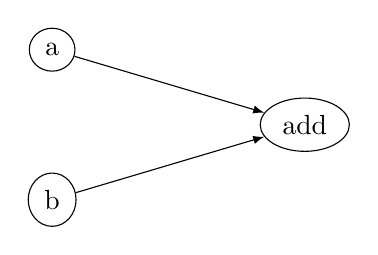
\begin{tikzpicture}[>=latex,line join=bevel,]
  \node (a) at (27.0bp,72.0bp) [draw,ellipse] {a};
    \node (add) at (117.95bp,45.0bp) [draw,ellipse] {add};
    \node (b) at (27.0bp,18.0bp) [draw,ellipse] {b};
    \draw [->] (b) ..controls (61.417bp,28.218bp) and (72.527bp,31.516bp)  .. (add);
    \draw [->] (a) ..controls (61.417bp,61.782bp) and (72.527bp,58.484bp)  .. (add);
  \end{tikzpicture}
  \caption[easygraph]{An easy computational graph}
  \label{fig:easygraph}
\end{figure}

The code to build the graph of Figure \ref{fig:easygraph} using the
TensorFlow Python API is

\begin{minted}{python}
  >>> import tensorflow as tf
  >>> a = tf.placeholder(tf.float32)
  >>> b = tf.placeholder(tf.float32)
  >>> add = tf.add(a, b)
  >>> add
  <tf.Tensor 'add:0' shape=<unknown> dtype=float32>
\end{minted}

\section{Keras}
\label{sec:keras}

Keras is a high level library for building Machine Learning models. It consists
of a simple API and bindings for a backend of choice, most notably TensorFlow.
When you use the library, you're encouraged to use \emph{layers} instead of
plain tensors. In fact the whole concept of TensorFlow tensors is hidden away by
the library abstractions. To implement your model you stack layers. For example,
you would stack a \texttt{Dense} layer and an \texttt{Activation} one to
implement a simple neural network.

\begin{minted}{python}
  from keras.models import Sequential

  model = Sequential([
    Dense(batch_input_shape=(None, 784), 10),
    Activation('softmax')
  ])
\end{minted}

Under the hood, a \texttt{Layer} is simply a callable object whose
\texttt{\_\_call()\_\_} method takes a TensorFlow tensor \texttt{X} and
manipulates it. For example a simple custom one would be
\begin{minted}{python}
  from keras.engine.base_layer import Layer
  import tensorflow as tf

  class Add42(Layer):
      def __init__(self):
          self.fortytwo = tf.constant(42)

      def __call__(self, X):
          return tf.add(X, self.fortytwo)
\end{minted}

While the idea is clean and beginner friendly, at the time of this writing the
abstraction can become leaky when things goes wrong, needing the programmer to know
about TensorFlow computational graphs to debug her program successfully.

\section{CleverHans}
\label{sec:cleverhans}

CleverHans is a library written by Google for building adversarial examples. It
implements a variety of attacks against neural networks (FGS, T-FGS, Carlini and
Wagner, ...) and it's compatible with models built with Keras. It uses the same
computational graphs of TensorFlow to generate adversarial examples; again, as
you use the library more and more understanding computational graphs becomes a
necessity.

\section{Scikit-learn}
\label{sec:sklearn}

Scikit-learn is a Python library written by Google providing a number of models,
learning algorithms and other utilities for Machine Learning. It's perfect for
fast prototyping as it uses a simple and consistent API and handles numpy arrays
or even Python lists.

I've used scikit-learn to borror a couple of decomposition algorithms (PCA, FastICA, ...)
without having to implement them. This required a bit of reasoning as reusing scikit-learn algorithms on
TensorFlow graphs was not straightforward.

  %%%%%%%%%%%%%%%%%%%%%%%%%%%%%%%%%%%%%%%%%%%%%%%%%%%%%%%%%%%%%%%%%%%%%%%%
\chapter{Training Models}
%%%%%%%%%%%%%%%%%%%%%%%%%%%%%%%%%%%%%%%%%%%%%%%%%%%%%%%%%%%%%%%%%%%%%%%%

Before running experiments on how ML models can be \emph{shielded}
against adversarial examples we had to create and train them.

\section{Motivation}
\label{sec:motivation}
As we're training a variety of models it's useful to find a strategy to
find an appropriate number of epochs to train the model for. Fixing a
number of epochs (say 500) and train all the models for that same
number of epochs feels \emph{cheesy}: some models can learn faster,
other slower, and you can end up comparing models that are at different
stage in their learning phase.

What we did was trying to \emph{understand} when the model has done
learning and stop training there. We used two approaches/heuristics
that are described in the following sections.

Note that trying to make the model learn better we reduced the learning
rate on plateau: if for a fixed number of epochs the accuracy on the
validation set does no longer improve, the learning rate is reduced.
This is known to help models to move on when the gradient descent
algorithm is stuck somewhere.

To make our experiments here we used a fully-connected neural network
with 2 layers of 100 hidden neurons each and 10 output neurons --
\emph{FC-100-100-10}. This structure is the same described in ???,
which is the paper we got inspiration from. ??? trained FC-100-100-10
for 500 epochs and we assume they chose that number as it gave them the
best results on the test set.

What we want to do is to empirically prove that we can achieve the
same accuracy on the test set without training FC-100-100-10 for
exactly 500 epochs but instead stopping training when the model stops
learning according to at least one of our heuristics.

\section{EarlyStopping}
\emph{EarlyStopping} is one of the two heuristics. It's already
implemented by Keras as a Callback. It checks if over a specified
number of epochs (the \emph{patience}) a specified metrics stopped
improving. When that happens the model is asked to stop training there.
We set a \emph{patience} of 60 epochs as on Google Cloud Platform 1
epochs runs is ~1 second; a patience of 60 epochs means that the model
didn't improve for a whole minute.

\section{StopOnStableWeights}
\emph{StopOnStableWeights} is the second heuristic. It has to be
implemented from scratch. This heuristic collects data on model's
weights over a specified number of epochs called the \emph{patience}.
Then, the same weight over different epochs is checked: if it has a
small standard deviation maybe it's getting stable. If the maximum of
these standard deviation is below a certain threshold we conclude the
model's weights are getting stable, hence the model is stopping
learning.

\section{Data obtained}
We obtained the following data:
\begin{itemize}
\item
  Model trained for 1000 epochs: accuracy on the test set of 97.71\%
\item
  Model trained for 500 epochs: accuracy on the test set of 97.55\%
\item
  Model trained for 500 epochs, reducing learning rate on plateau after
  30 epochs: accuracy on the test set of 97.47\%
\item
  Model trained for -1 epochs, stopping after accuracy on the
  validation set stopped improving for 60 epochs: accuracy on the test
  set of 97.44\% (trained for 424 epochs)
\item
  Model trained for -1 epochs, stopping as model weights had a maximum
  standard deviation of 0.5 over 60 epochs: accuracy on the test set of
  97.66\% (trained for 614 epochs)
\item
  Model trained for -1 epochs, stopping after accuracy on the
  validation set stopped improving for 60 epochs, reducing learning
  rate on plateau after 30 epochs: accuracy on the test
  set of 97.18\% (trained for 510 epochs)
\item
  Model trained for -1 epochs, stopping as model weights had a maximum
  standard deviation of 0.5 over 60 epochs, reducing learning
  rate on plateau after 30 epochs: accuracy on the test set of
  97.6\% (trained for 514 epochs)
\end{itemize}

\section{Conclusion}
From the above results the best approach seems to be using the
\emph{StopOnStableWeights} heuristics with a patience of 60 epochs,
reducing the learning rate on plateau after 30 epochs.

In the following chapters we'll use this setting for training models,
even when they're no longer the FC-100-100-10 used here.

  %%%%%%%%%%%%%%%%%%%%%%%%%%%%%%%%%%%%%%%%%%%%%%%%%%%%%%%%%%%%%%%%%%%%%%%%
\chapter{Reconstruction or retraining?}
%%%%%%%%%%%%%%%%%%%%%%%%%%%%%%%%%%%%%%%%%%%%%%%%%%%%%%%%%%%%%%%%%%%%%%%%

As we're testing different filter techniques it's important that we
understand how we're implementing these techniques in our models as
defenses.

\section{Motivation}
\label{sec:motivation}
There are at least two different fashions to integrate a
filter/decomposition technique in our models. We can either add a layer
to a pre-trained model and use it only \emph{after} training, or we can
add a layer to a pre-trained model and re-train the network after this
layer has been added. In the latter case, the model has been trained
only on filtered input, while in the former it does not. Following
lexicon used in ???, we named the first technique as
\emph{reconstruction} and the second one \emph{retraining}.

There's another alternative which is to initialize the model, add the
filter layer then train the network while it's still freshly
initialized. It basically consists in making the network never to see
unfiltered input. This seemed to make things so much better for the
attacker than both reconstruction and retraining that we just avoided
to compare it with the other approaches. Instead when it comes to
reconstruction and retraining who is better is not that clear. We did
some measurements to better understand it.

\section{How did we perform the comparison}

We built and train models using both reconstruction and retraining. We
had now two families of models. For example, for FC-100-100-10 with a
filter layer implementing PCA retaining 80 components we had one model
trained using reconstruction and another trained using retraining.

We attacked each model using Fast Gradient Sign obtaining a curve
saying what was the adversarial success score as $\eta$ increases --
where $\eta$ is the freedom given to the attacker: the more the freedom
the easier is to forge an input. Then, we paired each model trained
using reconstruction with the same model trained using retraining. We
computed the average value of the curve obtained subtracting the curve
for retraining from the curve for reconstruction. At last we computed
the average for the set of pairs, getting what is the average difference
between reconstruction and retraining.

\section{Data obtained}
We obtained that retraining is only 1\% more effective than reconstruction
when it comes to protect models from adversarial input.

\section{Conclusion}
While implementing retraining defense is not hard we concluded the
difference is not significant enough and decided to stick with
reconstruction which is a clearer solution -- it allows us to think about
filter techiniques without worrying about how that impacts on training.

  %%%%%%%%%%%%%%%%%%%%%%%%%%%%%%%%%%%%%%%%%%%%%%%%%%%%%%%%%%%%%%%%%%%%%%%%
\chapter{Image filters as a defense against adversarial input}
%%%%%%%%%%%%%%%%%%%%%%%%%%%%%%%%%%%%%%%%%%%%%%%%%%%%%%%%%%%%%%%%%%%%%%%%

In this chapter we'll test a couple of image filters against
adversarial input. The intuition behind the idea of filtering the image
is that to forge an adversarial input the attacker will try to put
little noise distributed in the image. As these filters highlight the
\emph{important} features of an image we hope they cut out the noise
introduced by the attacker.

For each of the filters tested in this chapter we can set its
parameters such that it can be more or less destructive in regards of
the original information. Intuitively the more invasive the filter the
better will be the defense. Unfortunately the better the defense the
more the lost accuracy too: two different images can be confused as the
same image for the model as the information that distiguished the two
images is now potentially lost. That means that the \emph{best} filter
will be the one that provides the best defense given the accuracy lost
by the model is not \emph{too much}.

<<SHOULDNT WE WRITE AN ATTACK CHAPTER?>> As a baseline we performed an
attack of Fast Gradient Sign with its parameter $\eta$ set to 0.1. We
chose that value for $\eta$ as it's a median value between a
non-effective attack -- when $\eta$ equals 0 -- and an attack that's
mostly unstoppable -- when $\eta$ is greater than 0.25.

<<INSERT 3 IMAGES OF THE SAME INPUT AS ETA INCREASES>>

In our \emph{gray-box} setting we measured an accuracy on the MNIST
test set of 97.39\% and a probability of success for the attacker of
81\%. Again, we expected these quantities to go down as we increase the
\emph{power} of the filter technique: while we try to stop the attacker
we have to reduce the accuracy of the model too.

\section{Principal Component Analysis}

<<WRITE GENERAL STUFF ON PCA>>

We tried the following setting for PCA: retain all the components of an
image (784 pixels), 331 of them, 100 of them, 20 and 10 components.

\begin{itemize}
  \item Retaining all the 784 components: accuracy 97.38\%, adversarial
    success score 82\%.
  \item Retaining 331 principal components: accuracy 97.52\%,
    adversarial success score 71\%.
  \item Retaining 100 principal components: accuracy 97.48\%,
    adversarial success score 44\%.
  \item Retaining 20 principal components: accuracy 94.18\%,
    adversarial success score 23\%.
  \item Retaining 10 principal components: accuracy 83\%, adversarial
    success score 22\%.
\end{itemize}

Of all these setting the best result is achieved when we retained 100
components. The accuracy on the MNIST test set is pretty the same (in
fact, it's even increased with the help of the filter) and the
adversarial success score is halved: from the original probability of
81\% to 44\%. When we're comparing PCA with other image filters we'll
consider this setting of 100 components.


% This ensures that the subsequent sections are being included as root
% items in the bookmark structure of your PDF reader.
%% \bookmarksetup{startatroot}
%% \backmatter

%%   \begingroup
%%     \let\clearpage\relax
%%     \glsaddall
%%     \printglossary[type=\acronymtype]
%%     \newpage
%%     \printglossary
%%   \endgroup

%%   \printindex
%%   \printbibliography

\end{document}
